\chapter{Trabalhos Relacionados}
\label{ch:relacionados}

Esta seção apresenta trabalhos relacionados com o modelo proposto, bem como uma comparação entre os mesmos. Foram escolhidos trabalhos que tivessem como foco a adaptação de um perfil de entidade de acordo com as ações tomadas pela mesma. Como não pode ser encontrado nenhum modelo que tivesse o foco pretendido para este trabalho (montagem de um perfil através de inferência em trilhas), foram escolhidos modelos que tivessem uma ou mais características que se farão úteis para o modelo deste trabalho.

Os trabalhos apresentados utilizam o conceito de modelo e perfil de usuário ao invés de modelo e perfil de entidade, que é o termo utilizado neste trabalho. Assim sendo, os termos modelo e perfil de usuário serão utilizados quando apropriado.

\section{\citetexto{pelep}}

O projeto PeLeP, apresentado por \citetexto{pelep}, integra a utilização de perfis aperfeiçoados automaticamente com ambientes de educação ubíqua.

\citetexto{barbosa05} compreendem Educação Ubíqua como sendo processos educacionais que ocorrem em qualquer lugar, a qualquer tempo e com qualquer dispositivo, de forma contínua, contextualizada e integrada ao cotidiano do aprendiz. Desta forma, o conhecimento presente no dia-a-dia das mais diferentes formas e em diferentes locais podem ser relacionados com processos educacionais direcionados aos aprendizes.

O PeLeP, cujo modelo é mostrado na Figura~\ref{fig:pelep1}, é dedicado ao gerenciamento de perfis de aprendizes em um ambiente ubíquo de ensino e aprendizagem. O modelo administra os perfis automaticamente, inferindo informações através do histórico do aprendiz. As alterações realizadas no perfil refletem o comportamento do aprendiz no ambiente ubíquo, levando em consideração o seu modelo de mobilidade e de contexto.

\begin{figure}
  \centering
  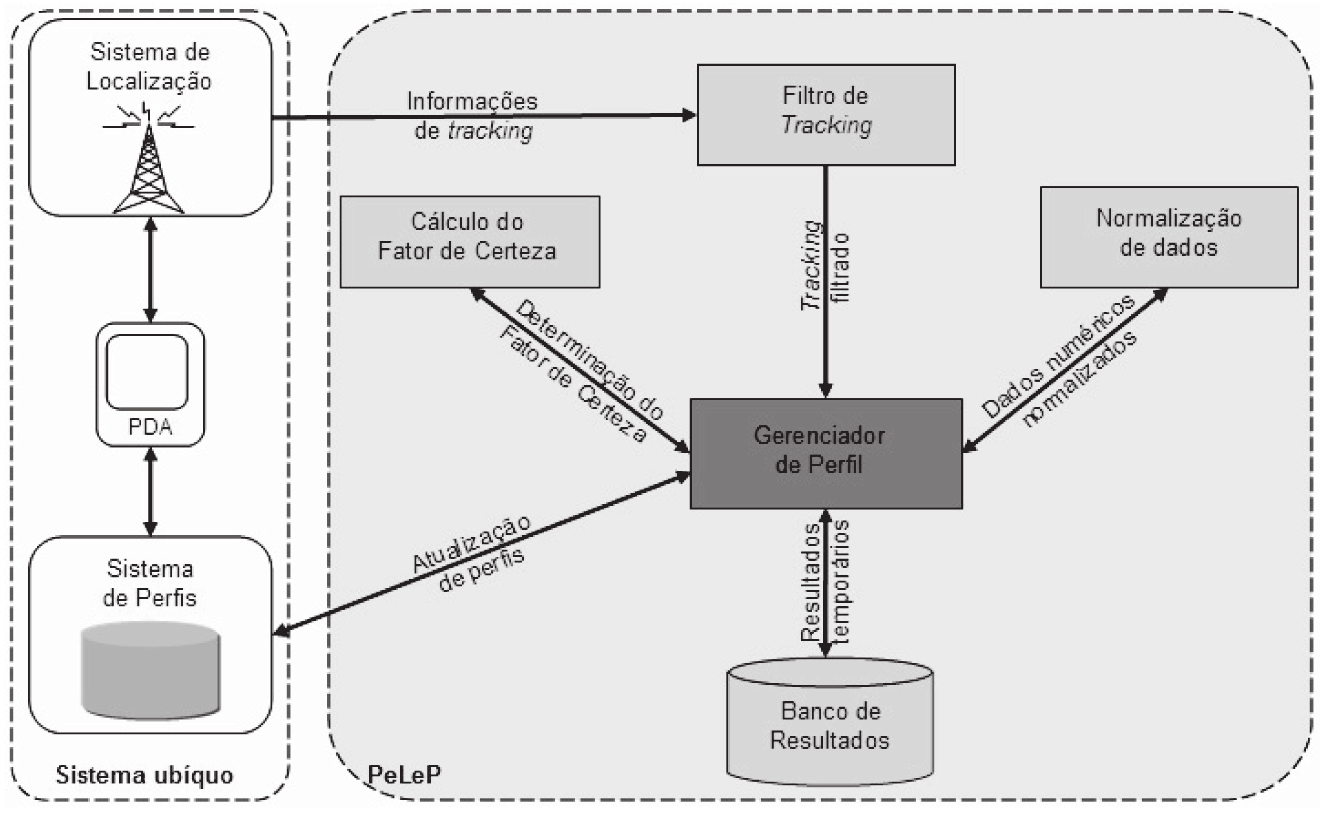
\includegraphics[width=0.8\textwidth]{imagens/pelep1.png}
  \caption[Arquitetura do PeLeP]{Arquitetura do PeLeP \cite{pelep}}
  \label{fig:pelep1}
\end{figure}

No PeLeP, o Perfil do Aprendiz consiste em um perfil contendo campos pré-definidos, voltados para o ambiente de educação ubíqua. Os campos são distribuídos nas seguintes categorias: identificação, objetivos, agenda, segurança, relacionamentos, competências e preferências. 

É realizado um acompanhamento ({\em tracking}) do histórico do aprendiz, onde são armazenados os contextos visitados pelo usuário, bem como os conteúdos, dispositivos e aplicativos utilizados em cada contexto. Os valores relativos das variáveis numéricas recebidas no {\emph tracking} são regularizados através de um processo de normalização de amplitude. Como diferentes valores podem ter diferentes impactos para a determinação da preferência de um usuário, calcula-se o Fator de Certeza ($FC$), de acordo com a equação~\ref{eq:pelep-fc}, onde $f_i$ é o valor normalizado para o fator, $p_i$ o seu percentual, e $n$ o número de fatores considerados.

\begin{equation}
  FC = \frac{\frac{\displaystyle\sum_{i=0}^n f_i p_i}{100}}{n}
  \label{eq:pelep-fc}
\end{equation}

O fator tempo também é levado em consideração, onde Fatores de Certeza mais antigos têm um impacto menor. Assim, por exemplo, se o usuário trocar o seu aplicativo preferido, à medida que o tempo for passando o impacto do aplicativo anterior será cada vez menor.

O processo de atualização do modelo do aprendiz é então realizado através de regras pré-definidas, que levam em conta as ocorrências e o seu fator de certeza. As regras suportam conclusões a partir de evidências antecedentes, e cada categoria de informação possui regras diferentes.

O PeLeP foi validado através da integração com o Local ({\em Location and Context-Aware Learning}), um sistema de educação ubíqua sensível a contexto \cite{barbosa11}.

%%%%%%%%%%%%%%%%%%%%%%%%%%%%%%%%%%%%%%%%%%%%%%%%%%%%%%%%%%%%%%%%%%%%%%%%%

\section{\citetexto{chellouche10}}

O modelo de \citetexto{chellouche10} busca resolver as dificuldades atuais no desenvolvimento de aplicativos para dispositivos móveis, uma vez que os mesmos possuem uma grande variedade de resolução, memória, poder computacional, entre outros. Além disso, a qualidade da conexão de um usuário pode variar significativamente, e isto também deve ser levado em consideração no desenvolvimento.

O conjunto de informações que caracteriza um usuário é chamada de Perfil de Usuário. Com a intenção de compartilhar o contexto do usuário entre serviços e minimizar as mudanças no desenvolvimento de aplicações sensíveis a contexto, os autores propõem como solução um {\em middleware} que gerencia o perfil de um usuário dinamicamente e supre às aplicações todas as informações que elas podem precisar durante o período de adaptação.

O perfil do usuário é constituído por seu contexto, onde a definição de contexto utilizada é aquela dada por \citetexto{dey2001}, na qual contexto refere-se a qualquer informação que pode ser utilizada para caracterizar a situação de uma entidade. Assim, o perfil de usuário é dividido em cinco componentes:

\begin{itemize}
  \item Perfil geral: refere-se às informações básicas, como nome, endereço, telefone, idade, sexo, entre outros;
  \item Perfil do dispositivo: contém informações a respeito dos dispositivos do usuário, tais como marca, capacidade, sistema operacional, entre outros;
  \item Perfil de rede: descreve as redes às quais o usuário pode se conectar, com suas características;
  \item Perfil dos serviços: registra as informações a respeito de serviços, como nome, versão, porta e conteúdo;
  \item Perfil de contexto: contém informações a respeito do ambiente do usuário, como hora, data e localização, aplicações em execução e banda disponível. É considerada a parte dinâmica do perfil, composta por dados voláteis.
\end{itemize}

O {\em middleware} é apresentado segundo ilustrado na Figura~\ref{fig:chellouche1}, sendo composto dos seguintes módulos:

\begin{figure}
  \centering
  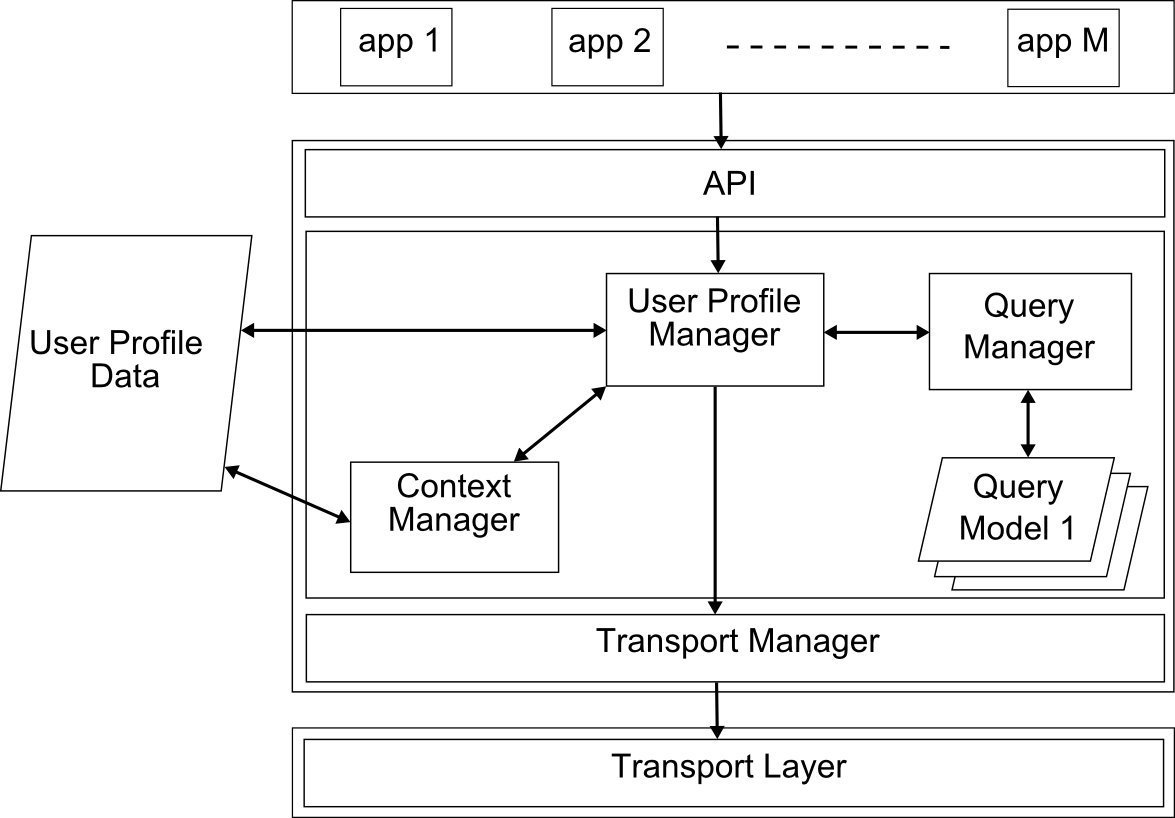
\includegraphics[width=0.8\textwidth]{imagens/chellouche1.png}
  \caption[Arquitetura do {\em middleware} de Chellouche et al]{Arquitetura do {\em middleware} de \citetexto{chellouche10}}
  \label{fig:chellouche1}
\end{figure}

\begin{itemize}
  \item Gerenciador de perfil de usuário: módulo central da arquitetura, que interage com todos os outros módulos com o objetivo de construir o perfil correto;
  \item Gerenciador de contexto: monitora o ambiente, coletando informações com o objetivo de atualizar a parte dinâmica do perfil;
  \item Gerenciador de consultas: módulo responsável por validar e salvar um modelo de consulta para cada aplicação;
  \item Gerenciador de trasporte: faz a comunicação do perfil de usuário para a aplicação;
  \item API: constitui o ponto de interface entre as aplicações e o \em{middleware}.
\end{itemize}

O perfil é construído seguindo o fluxo apresentado na Figura~\ref{fig:chellouche2}. A aplicação solicita os dados ao gerenciador de perfis, através da API, que por sua vez repassa a solicitação ao gerenciador de consultas. Ao mesmo tempo, o gerenciador de contextos é informado que a aplicação está em execução e passa a atualizar o gerenciador de perfis com as informações atualizadas. O perfil de usuário é criado e enviado ao gerenciador de transporte, que retorna o perfil solicitado à aplicação solicitante.

\begin{figure}
  \centering
  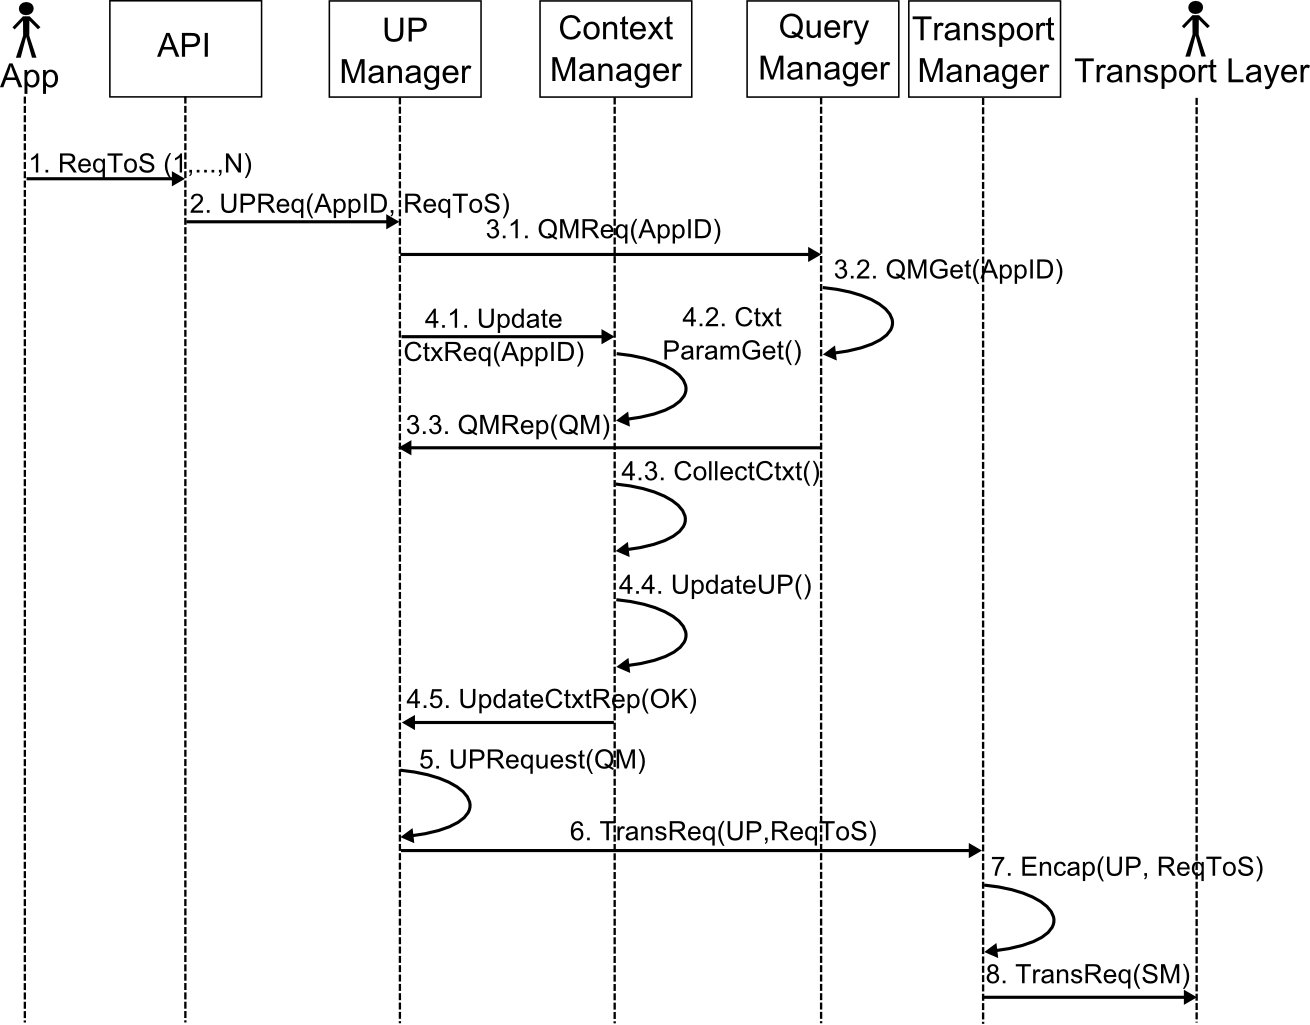
\includegraphics[width=0.8\textwidth]{imagens/chellouche2.png}
  \caption[Construção de perfil]{Construção de perfil \cite{chellouche10}}
  \label{fig:chellouche2}
\end{figure}

%%%%%%%%%%%%%%%%%%%%%%%%%%%%%%%%%%%%%%%%%%%%%%%%%%%%%%%%%%%%%%%%%%%%%%%%%%

\section{\citetexto{niederee04}}

O artigo apresentado por \citetexto{niederee04} busca responder três indagações, que são apresentadas como sendo os três desafios básicos da personalização:

\begin{itemize}
  \item como modelar o usuário e sua situação de modo extensível e unificado, de forma que este modelo possa ser interpretado e usado para personalização por diferentes sistemas?
  \item como coletar dados para preencher e atualizar perfis de usuário a partir das interações do usuário com diferentes sistemas baseados em um modelo de contexto de usuário unificado?
  \item como habilitar conceitualmente e tecnicamente diferentes sistemas a fazer uso dos perfis de usuário coletados para aperfeiçoamento do suporte ao usuário?
\end{itemize}

Os autores apresentam como resposta a estas indagações um modelo denominado UUCM, que tem como objetivo modelar características do usuário e de seu contexto. O conceito de contexto utilizado é aquele apresentado por \citetexto{benerecetti00}, no qual o contexto pode ser pensado como as informações extras, geralmente implícitas (como associações, fatos, suposições), que podem ser utilizadas para compreender plenamente uma interação, comunicação ou representação de conhecimento.

A abordagem para a modelagem unificada de contextos de usuário é proposta em dois níveis. No nível \emph{abstrato}, são definidos os blocos básicos de construção: contexto de usuário, facetas do modelo de usuário, propriedades principais e dimensões do modelo de usuário. O termo faceta representa as diferentes características do usuário.  Este nível define um metamodelo para as dimensões e facetas concretas utilizadas na descrição do modelo de contexto de usuário. Para que a abordagem de personalização multi-sistema seja válida, é necessário que este metamodelo de contexto de usuário seja publicado como uma ontologia compartilhada, e que todos os participantes utilizem este modelo.

No nível \emph{concreto}, um conjunto de dimensões e facetas são definidos. As facetas e dimensões são descritas como parte de uma ontologia adicional que é compartilhada pelos componentes envolvidos na personalização multi-sistemas.

\begin{figure}
  \centering
  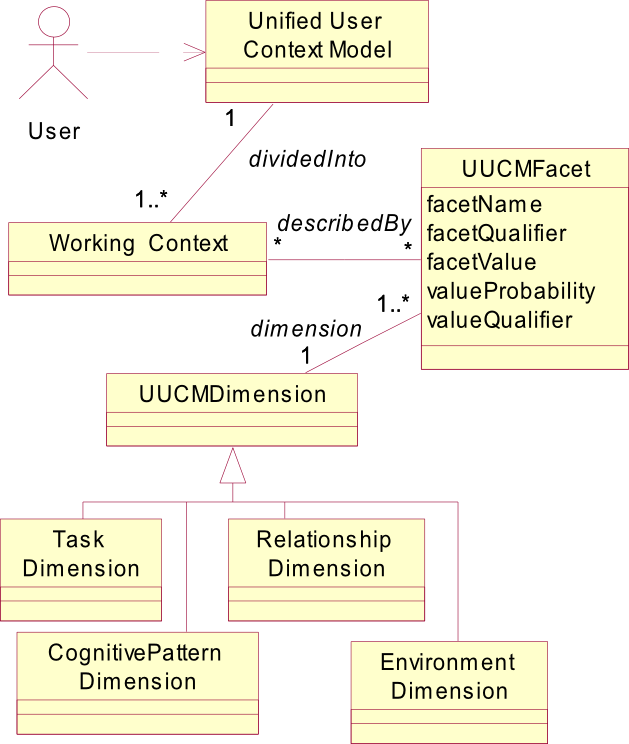
\includegraphics[width=0.5\textwidth]{imagens/niederee1.png}
  \caption[Modelo do UUCM]{Modelo do UUCM \cite{niederee04}}
  \label{fig:niederee1}
\end{figure}

O modelo do UUCM é apresentado na Figura~\ref{fig:niederee1}. Segundo o modelo, um perfil de usuário ({\em Unified User Context Model}) é dividido em um conjunto de contextos de trabalho ({\em Working Context}), onde cada contexto é descrito por um conjunto de facetas ({\em UUCM Facet}). Cada faceta é vinculada a uma dimensão ({\em UUCMDimension}).

O UUCM apenas define o método através do qual o perfil de contexto de usuário é descrito e estruturado para personalização multi-sistema. Para a descrição de perfis de contexto concretos, o UUCM utiliza ontologias (ou vocabulários) para as dimensões, facetas e valores de faceta.

As seguintes dimensões são utilizadas:

\begin{itemize}
  \item Cognitiva: ({\em CognitivePattern}): descreve as dimensões cognitivas do usuário, tais como áreas de interesse, competências e preferências;
  \item Tarefa: ({\em Task}): descreve os objetivos do usuário quando ele interage com sistemas. Esta dimensão utiliza dados tais como tarefa atual, papel do usuário na tarefa e histórico da tarefa;
  \item Relacionamentos: ({\em Relationship}): armazena as entidades com as quais o usuário tem alguma relação;
  \item Ambiente: ({\em Environment}): parâmetros que são tipicamente utilizados para abordagens sensíveis a contexto, tais como tempo, localização, dispositivo e linguagem.
\end{itemize}

O perfil de usuário do UUCM é codificado como um RDF Schema\cite{rdf}, ampliado com expressões OWL.

O modelo inclui ainda o conceito de Passaporte de Contexto. O passaporte de contexto é uma representação compacta do modelo de contexto atual do usuário para a personalização multi-sistemas. Ele contém informações ontologicamente arranjadas a respeito dos padrões cognitivos (habilidades, interesses, etc), o ambiente (data, local, dispositivo usado) e sua rede pessoal de pessoas e relacionamentos envolvidos.

Para utilizar o passaporte de contexto em um ambiente de personalização multi-sistemas, o usuário ``apresenta'' o passaporte ao sistema que o usuário deseja utilizar. Como o passaporte está vinculado a uma ontologia compartilhada, é possível que o sistema consiga interpretar parcialmente o passaporte através de uma arquitetura mediadora. Como resultado, dois fluxos são possíveis: (i) do passaporte para o sistema, auxiliando o sistema a compreender o contexto do usuário, e (ii) do sistema para o passaporte, realizando alterações nas informações de contexto do usuário.

%%%%%%%%%%%%%%%%%%%%%%%%%%%%%%%%%%%%%%%%%%%%%%%%%%%%%%%%%%%%%%%%%%%%%%%%%%

\section{\citetexto{kim08}}

\citetexto{kim08} apresentam um {\it framework} para gerenciamento de perfis baseado em {\it Web Services} para fornecer serviços personalizados. Os autores compreendem gerenciamento de perfil como sendo a coleta de um conjunto de informações necessárias para prover aos usuários cinco tipos de serviço personalizado: (i) configuração de perfil, (ii) criação de perfil, (iii) troca de perfil, (iv) processamento de perfil e (v) serviço de perfil.

O {\it framework} é montado de acordo com a Figura~\ref{fig:kim08_b}. A comunicação entre os módulos é feita através de {\it Web Services}, de modo a poder operar de forma distribuída entre várias plataformas e dispositivos.

\begin{figure}
  \centering
  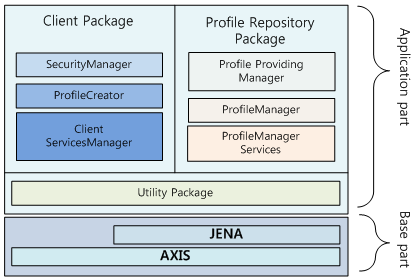
\includegraphics[width=0.6\textwidth]{imagens/kim08_b.png}
  \caption{Framework de perfis \cite{kim08}}
  \label{fig:kim08_b}
\end{figure}

A configuração de perfil configura os perfis em dois tipos: perfis básicos, requeridos para todos os tipos de serviço, e perfis de serviço, configurados diferentemente para cada tipo de serviço. O tipo de perfil define o tipo de informação que irá conter cada perfil.

A criação de perfil é a tecnologia que permite que clientes e provedores de serviço criem os perfis. A criação dos perfis é feita através de um conjunto de componentes, de acordo com a Figura~\ref{fig:kim08_a}. O Gerenciador de Criação cria o perfil, com base nos Arquivos de Template de Perfil, que é então codificado pelo Gerenciador de Segurança, num processo coordenado pelo Gerenciador de Serviços de Perfil. Toda a comunicação entre os módulos ocorre via {\it Web Services}.

\begin{figure}
  \centering
  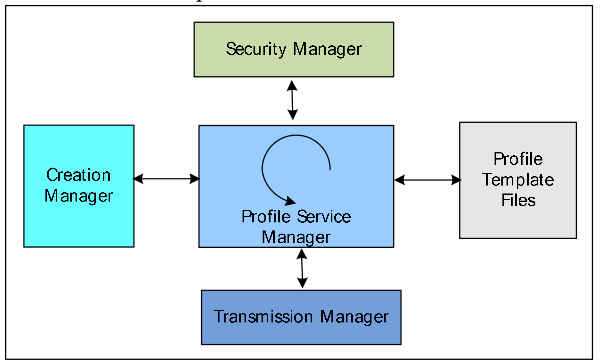
\includegraphics[width=0.6\textwidth]{imagens/kim08_a.png}
  \caption{Mecanismo de Criação de Perfis \cite{kim08}}
  \label{fig:kim08_a}
\end{figure}

Troca de perfis é o processo através do qual um perfil é enviado pelo servidor ao cliente. O processamento do perfil classifica os perfis transferidos pelos clientes através de regras e os armazena em uma base de dados. Os serviços de perfil extraem os perfis do repositório e os fornecem aos provedores de serviço quando os mesmos os requisitam.
%%%%%%%%%%%%%%%%%%%%%%%%%%%%%%%%%%%%%%%%%%%%%%%%%%%%%%%%%%%%%%%%%%%%%%%%%%

\section{\citetexto{tao11}}

No artigo apresentado por \citetexto{tao11}, os autores avaliam que, embora ontologias venham sendo cada vez mais uilizadas como modelo de descrição e formalização de conhecimento, a maioria dos modelos utiliza somente as informações de uma base de conhecimento global ou informações locais de usuário para montar um perfil de usuário. Desta forma, é proposto um modelo de ontologia sobre perfis de usuários que compõe-se tanto a partir de uma base de conhecimento global quanto de repositórios locais de usuários.

De acordo com os autores, ontologias personalizadas são um modelo de conceitualização que formalmente descrevem e especificam o conhecimento de fundo do usuário. Por exemplo, quando o usuário busca pelo tópico "New York" em um agente de buscas, a informação demandada é diferente para usuários de negócios e turistas. A expectativa pode ser diferente até mesmo para o mesmo usuário fazendo a mesma busca em contextos diferentes (um usuário de negócios pode estar fazendo a busca para uma viagem de negócios ou a lazer, por exemplo). Desta forma, o modelo conceitual do usuário pode mudar de acordo com a sua necessidade.

A primeira base de informação é uma representação de conhecimento global. A base utilizada pelo modelo é a {\it Library of Congress Subject Headings} (LCSH). A LCSH foi desenvolvida para organizar e consultar informações de um grande volume de coleções da Biblioteca do Congresso Americano. O sistema da LCSH possui três tipos de referência: ``termo amplo'', ``usado para'' e ``termo relacionado''. Estas referências e as ligações entre elas são usadas para construir o conhecimento de mundo necessário para a composição da ontologia.

A base de interesses de usuários é extraída através de uma ferramenta denominada {\it Ontology Learning Environment} (OLE). A ferramenta constrói a ontologia através da alimentação manual de informações pelo usuário. A ontologia classifica os assuntos alimentados pelo usuário em três tipos: (i) ``assuntos positivos'', (ii) ``assuntos negativos'' e ``assuntos neutros.'' Assuntos positivos são conceitos relevantes para a informação necessária, e assuntos negativos são conceitos que resolvem interpretações ambíguas ou paradoxais. Assuntos neutros são aqueles que não tem relevância para a informação buscada.

\begin{figure}
  \centering
  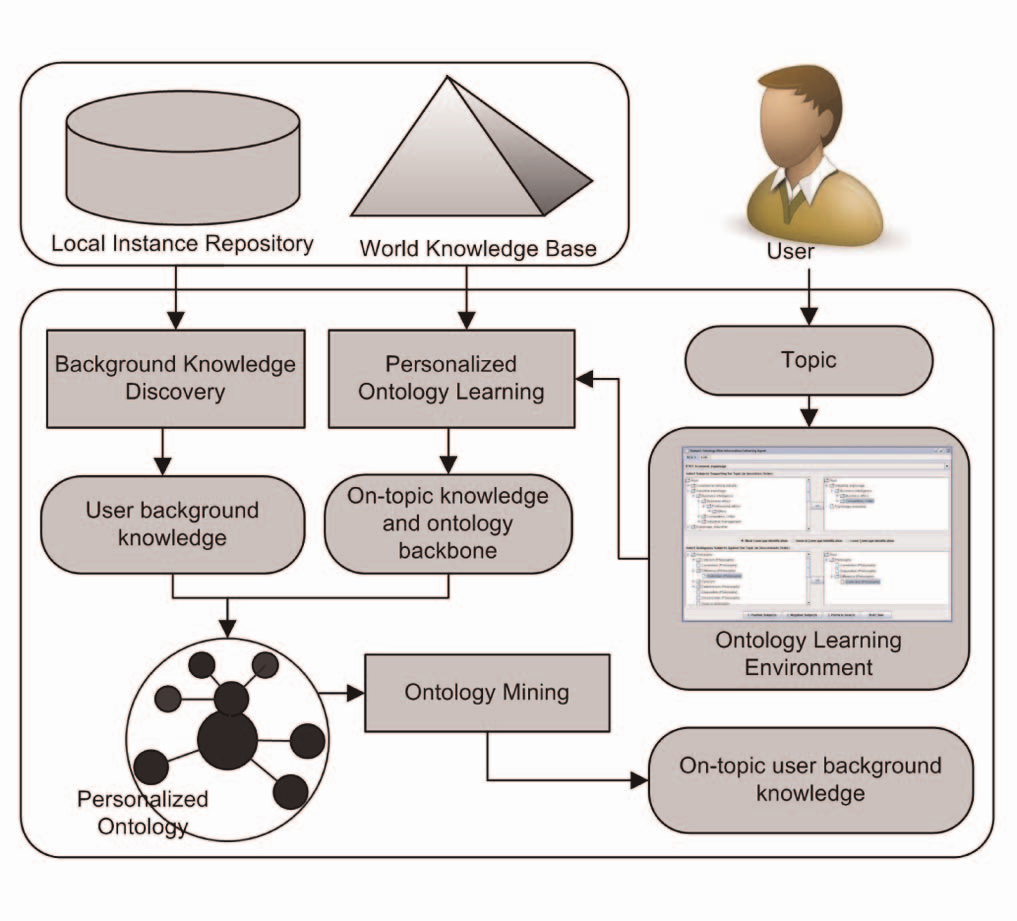
\includegraphics[width=0.6\textwidth]{imagens/tao11.png}
  \caption[Arquitetura do modelo de \citetexto{tao11}]{Arquitetura do modelo de \citetexto{tao11}}
  \label{fig:tao11}
\end{figure}

A Figura~\ref{fig:tao11} apresenta a arquitetura do modelo. O passo inicial do processo é a construção da ontologia, de acordo com um determinado tópico, utilizando como base as duas fontes de conhecimento (base de conhecimento global e as informações locais de usuário). A base de conhecimento local e as informações providas pelo OLE são utilizadas para gerar o conjunto de informações sobre o assunto que, unido ao {\it background} do usuário, são processados atraves de um processo chamado ``mineração de ontologia'', que gera o conhecimento de {\it background} do usuário a respeito de um determinado tópico.

%%%%%%%%%%%%%%%%%%%%%%%%%%%%%%%%%%%%%%%%%%%%%%%%%%%%%%%%%%%%%%%%%%%%%%%%%%

\section{\citetexto{razmerita11}}

\citetexto{razmerita11} apresenta o modelo OntobUMf ({\it Ontology-based User Modeling framework}), um {\it framework} para modelagem de usuários baseado em ontologia. O artigo defende que o gerenciamento de conhecimento (KM, ou {\it Knowledge Management}) são tarefas importantes para indivíduos e organizações, e que sistemas de gerenciamento de conhecimento (KMS) atuais focam no compartilhamento e criação de conteúdo que, por sua vez, leva à inovação tanto a nível individual quanto corporativo. Mais recentemente, o KM pessoal tem se tornado relevante, e foca na busca do indivíduo em encontrar, aprender, compartilhar conteúdo e socializar.

O modelo OntobUMf busca unir o KM tradicional com o KM pessoal através da personalização de um KMS, de modo a permitir a customização de {\it interfaces} e adaptação da funcionalidade, estrutura, conteúdo e modularidade, aumentando assim a relevância para usuários individuais.

\begin{figure}
  \centering
  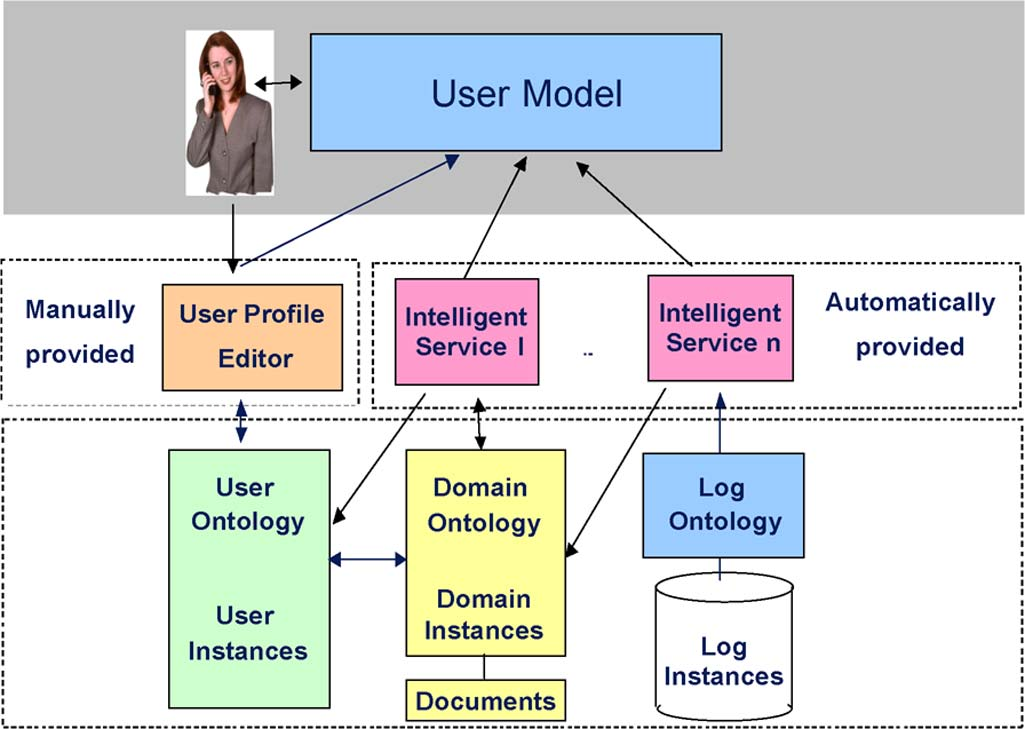
\includegraphics[width=0.6\textwidth]{imagens/razmerita11.png}
  \caption{Arquitetura do modelo OntobUMf}
  \label{fig:razmerita11}
\end{figure}

A Figura~\ref{fig:razmerita11} apresenta a arquitetura do modelo OntobUMf. OntobUMf é uma aplicação de três camadas: (i) {\it front end}, (ii) serviços e (iii) dados. A camada de {\it front end} é um conjunto de {\it interfaces} de usuário que permitem que o usuário acesse e atualize seu modelo de usuário ou perfil de usuário. 

A camada de serviços contém vários serviços inteligentes, tais como algoritmos de modelagem de usuários, mecanismos de personalização, entre outros. Os serviços possuem duas tarefas principais no sistema. A primeira é atualizar e manter o modelo de usuário tendo por base os dados de uso disponíveis do sistema através de um extrator de categoria, que é composto por um conjunto de mecanismos para modelagem das características dos usuários que estão interagindo com o sistema. A segunda tarefa é fornecer um conjunto de serviços personalizados baseados nas características dos usuários.

A camada de dados inclui dados de usuários relacionados a dados específicos de domínio. Ontologias capturam o conceito e as relações entre os conceitos descrevendo diferentes recursos disponíveis no sistema. OntobUMf possui três ontologias. A ontologia de usuários estrutura as características dos usuários, classificando-as em conceitos, subconceitos, propriedades e relacionamentos. A ontologia de domínios descreve o domínio de conhecimentos e os relacionamentos entre os diferentes conceitos. A ontologia de log define a semântica de interação do usuário com o sistema, descrevendo as ações do usuário e os eventos associados disparados pelo sistema.

A OntobUMf classifica os usuários de acordo com o nível de atividade, o tipo de atividade e nível de compartilhamento de conhecimento. Baseado no tipo de atividade, os usuários são classificados como ``leitores'', ``escritores'' ou ``espiões''. Baseado no nível de atividade, os eles são classificados como ``muito ativo'', ``ativo'', ``visitante'' e ``inativo''. Baseado no nível de compartilhamento de conteúdo, eles são classificados como ``inconsciente'', ``consciente'', ``interessado'', ``tentativo'' ou ``adotante''.


%%%%%%%%%%%%%%%%%%%%%%%%%%%%%%%%%%%%%%%%%%%%%%%%%%%%%%%%%%%%%%%%%%%%%%%%%%

\section{Considerações finais}

A Seção~\ref{sec:contribuicoes} apresenta uma comparação entre os trabalhos apresentados neste capítulo e o modelo que está sendo proposto nesta dissertação.

%\section{Considerações sobre os trabalhos relacionados}

%A Tabela~\ref{tab:comparacao} exibe um comparativo entre os trabalhos apresentados neste capítulo, onde os seguintes fatores são levados em consideração:
%
%\begin{itemize}
%  \item Interoperabilidade: considera se o modelo apresenta interoperabilidade -- caso positivo, se a mesma é sintática ou semântica;
%  \item Perfis dinâmicos: identifica se o modelo de perfil permite que os perfis sejam atualizados de acordo com eventos externos, sem a interferência do usuário;
%  \item Armazenamento: define onde ficam armazenados os perfis do usuário;
%  \item Sensíbilidade a contexto: considera se o contexto do usuário é levado em consideração na formação do perfil;
%  \item Utiliza trilhas: define se as trilhas do usuário são levadas em consideração na construção do perfil;
%  \item Domínio: identifica se o perfil é voltado para um domínio específico, ou se o mesmo permite que vários domínios possam ser utilizados.
%\end{itemize}

%\begin{table*}\centering\footnotesize
%  \begin{tabular*}{1\textwidth}{@{}lllllll@{}}
%    \toprule
%                                         & Interope-  & Perfis    & Armaze-  & Sensibilidade & Utiliza & \\
%    Trabalho                             & rabilidade & dinâmicos & namento  & a contexto    & trilhas & Domínio \\
%    \midrule
%    \citetexto{pelep}                    & Não        & Sim       & Servidor & Sim           & Parcial & Educação \\
%    \citetexto{chellouche10}             & Sintática  & Sim       & Servidor & Sim           & Não     & Serviços multimídia \\
%    \citetexto{niederee04}               & Sintática  & Sim       & Cliente  & Sim           & Não     & Genérico \\
%    \citetexto{tao11}                    & 
%    \citetexto{razmerita11}              & 
%    \citetexto{kim08}                    
%    \bottomrule
%  \end{tabular*}
%  \caption{Comparação entre os trabalhos apresentados}
%  \label{tab:comparacao}
%\end{table*}

%O PeLeP \cite{pelep} é um modelo que suporta o aperfeiçoamento automático do perfil do aprendiz em ambientes de educação ubíqua. Ele usa o histórico dos aprendizes nos contextos de um ambiente ubíquo para atualização dos perfis. O perfil do aprendiz no modelo é refinado e enriquecido através de inferências. As inferências são baseadas na mobilidade do aprendiz e no monitoramento das tarefas que ele executa nos contextos de um ambiente de educação ubíqua.
%
%O modelo apresentado por \citetexto{chellouche10} apresenta um {\em middleware} voltado para aplicações móveis que pode ser usado por diferentes aplicativos como um servidor central de perfis. Este modelo propõe como solução um {\em middleware} que gerencia o perfil de um usuário dinamicamente e supre às aplicações todas as informações que elas podem precisar durante o período de adaptação.
%
%O UUCM \cite{niederee04} é um modelo que pode ser utilizado para modelar as características de um usuário e seu contexto em ambientes de personalização de múltiplos sistemas. A proposta diz respeito a uma ontologia básica, baseada em contexto, a qual os sistemas podem estender, desde que os sistemas que usem este modelo concordem em uma ontologia básica.
%
%O modelo apresentado por \citetexto{tao11} apresenta a proposta de unir conhecimento global e repositórios locais, de modo a obter informações mais completas a respeito de um usuário. O modelo 
%
%
% Não encontrou-se nenhum modelo que ofereça suporte a estes pré-requisitos de forma genérica (isto é, para qualquer tipo de contexto) e, assim, este modelo busca suprir esta necessidade.
%
%Dos trabalhos avaliados, o PeLeP suporta o aperfeiçoamento automático do usuário, e o modelo apresentado por \citetexto{chellouche10} distribui um perfil unificado entre as aplicações. Já o UUCM apresenta uma ontologia básica de perfis que as aplicações podem estender, e que podem ser utilizadas por diversas aplicações, além de trabalhar em um domínio genérico. Cada um destes trabalhos apresenta alguma característica importante para o modelo que será apresentado no Capítulo~\ref{ch:modelo}, que possui ainda outras características que não estão presentes em nenhum dos trabalhos estudados, como o uso de trilhas para a extração das informações.
